\section{Practical 1 - Testing methodologies}
\label{sec:Prac1}
\subsection{Introduction}
The focus of this task is on using OCTAVE (the free sort-of MATLAB program) and doing some statistical operations. In later assignments you will make further use of these statistical functions, and perhaps reuse this code, in comparing and discussing results obtained in other practicals and projects (for example, correlation can be used in analysing gold standard results to higher-speed approximation result).

For installation and tips and tricks on using Octave, visit \href{http://wiki.ee.uct.ac.za/Octave}{The EE Wiki} (currently only accessible on the UCT Network - though you can use a VPN).

\textbf{Note:}\\
If you're doing a smaller installation of Octave, there are the libraries you require from Octave Forge:
audio ; control ; data-smoothing ; fixed ; ga ; gnuplot ; image ; integration ; oct2mat; plot ; signal ; sockets ; specfun ; splines ; statistics ; strings


\subsubsection{Correlation}
Correlation is a useful statistical function for comparing two datasets to judge how similar or different they are. The correlation function returns a correlation coefficient, r, between -1 and 1. A value of 1 for r implies perfect positive correlation, i.e. the two datasets are the same. Correlation of 0 implies there is no correlation (the two datasets behave totally differently). A correlation of -1 indicates a total opposite - for example if you compare vectors x to - x you get a correlation of -1. Generally if $|r| >= 0.8$ there is strong correlation, between 0.5 and 0.8 moderate weak, less that 0.5 is weak (towards no) correlation.

Pearson's correlation (which you can read more about on \href{https://en.wikipedia.org/wiki/Pearson_correlation_coefficient}{Wikipedia}) is implemented as follows:
\begin{equation}
\label{eqn:Pearson}
  r =
  \frac{ \sum_{i=1}^{n}(x_i-\bar{x})(y_i-\bar{y}) }{%
        \sqrt{\sum_{i=1}^{n}(x_i-\bar{x})^2}\sqrt{\sum_{i=1}^{n}(y_i-\bar{y})^2}}
\end{equation}

\subsubsection{Speed Up}
\begin{equation}
Speedup = \frac{T_{p1}}{T_{p2}}
\end{equation}
Where:\\
$T_{p1}$ = Run-time of original / non-optimal program\\
$T_{p2}$ = Run-time of optimised program

For obtaining a repeatable timing value, run each version (i.e. initial version and optimised version) of your programs more than once and discard the first measured time. You can, if you want to be complete, indicate what the initial speed up was and then the average speed up.

\subsubsection{Critical Section}
When measuring performance, it's important to ensure that you are only measuring the section of your algorithm that you need to measure. For example, if you are measuring the execution time of an audio filter, you should not be recording the time taken to open and close the files you are applying this filter to.

\subsection{Requirements}
You are required to run the following experiments:
\subsubsection{Measuring Execution Time of rand()}
White noise is often generated with GNU Octave’s random number generator \verb|rand()|, which generates uniformly distributed random values in the interval [0,1). To create a sound wave of the white noise, the \verb|wavwrite()| function in Octave is used. The \verb|wavwrite()| function expects values in [-1.0, 1.0), so the \verb|rand()| output must be multiplied by 2 and shifted down by 1. To generate 10 seconds white noise sampled at 48 kHz, the following instruction are called:
\begin{lstlisting}
white = rand(48000*10,1)*2-1;
\end{lstlisting}
And to generate a wave file for this noise, we use the \verb|wavwrite()| function as follows:
\begin{lstlisting}
wavwrite(white, 48000, 16, 'white_noise_sound.wav');
\end{lstlisting}

\textbf{NOTE:}\\
\verb|wavwrite| and \verb|wavread| were deprecated in Octave 5.1. If you're using Octave 5.1 or greater, you need to use \verb|audiowrite| and \verb|audioread|.
\begin{lstlisting}
audiowrite('w.wav', white, 48000, 'BitsPerSample', 16);
[y, fs] = audioread('w.wav', 16);
\end{lstlisting}

\subsubsection{White Noise Generator Script}
Next, write a function in a new file called \verb|createwhiten.m| that implements a function with a \textbf{for loop} that generates a white noise signal, one sample at a time, comprising N duration in seconds. You can assume that N will always be positive and a multiple of 10. The white noise must be sampled at either 48 kHz or 8 kHz. Name your function \verb|createwhiten(...)|. You need to use the \verb|rand()| function without arguments so that it will generate a single random value, and the main task is figuring out how to scale so that you create a suitable input to \verb|wavwrite(...)| as explained above. Call the function and check output size as follows:
\begin{lstlisting}
whiten = createwhiten(1000);
size(whiten);
\end{lstlisting}
should return:
\begin{lstlisting}
ans = 48000000 1
\end{lstlisting}
Check that the resulting wave/sound file gives the same sound as the white noise sound.wav generated above by generating the new sound file named white noise sound2.wav and playing it back.
\begin{lstlisting}
wavwrite(whiten, 48000, 16, 'white_noise_sound2.wav');
\end{lstlisting}

\subsubsection{Visual Confirmation of Uniform Distribution}
Confirm that you've created the sample correctly. Since it’s a big signal, let’s just look at the first 100 samples by plotting using a histogram function as follows:
\begin{lstlisting}
hist(whiten, 100, 1);
\end{lstlisting}
This should give image shown in Figure \ref{fig:octave_hist}:

\begin{figure}[H]
\centering
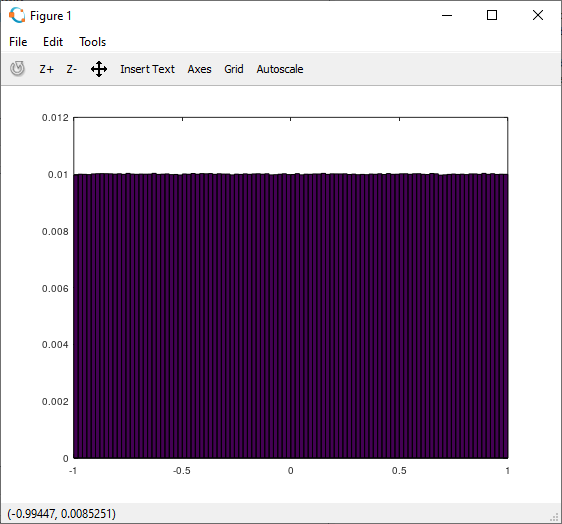
\includegraphics[width=0.6\columnwidth]{Figures/octave_hist}
\caption{Output of hist(whiten, 100, 1);}
\label{fig:octave_hist}
\end{figure}

\subsubsection{Timing Execution}
Now time how long it took to execute the script. Use the \verb|tic()| and \verb|toc()| functions as follows. Note that the call to tic is on the same line just before the function - this tends to have less delay between the start of the timer and starting the function. Of course, it is good practice to put it all in a script file.
\begin{lstlisting}
tic; white = rand(48000*1000, 1)*2 - 1; runtime = toc();
disp(strcat("It took: ", num2str(runtime*1000), " ms to run"));
\end{lstlisting}

Call the \verb|createwhiten(...)| function you created that does the same thing as the \verb|white = rand(48000*1000,1)*2 - 1;| statement that generate the white noise. Measure the time it took for your \verb|createwhiten(...)| function to run and show the timing difference (in milliseconds) and discuss the speed-up you have achieved (if any).

\subsubsection{Implementing Pearson's Correlation}
Implement the Pearson's correlation formula a new m file called it \verb|mycorr.m|. Provide your code in your report. Marks will be awarded on elegance of your code.

\subsubsection{Comparing Your Correlation Function to Octave}
The \verb|cor| function in OCTAVE performs a correlation operation. Compare your \verb|mycorr| results to the build-in cor function. First read the noise wave file using \verb|wavread(...)|, then you could, for example, use the following code to test your \verb|mycorr(...)| function as compared to Octave’s \verb|cor(...)|:
\begin{lstlisting}
x = wavread('white_noise_sound.wav');
y = x;
r1 = mycorr(x,y)
r2 = cor(x,y) # note that in some versions, this is called "corr"
disp(r2 - r1);
y(1) = 2; y(5) = -4; # i.e. fudge some of the value
r1 = mycorr(x,y)
r2 = cor(x,y)
disp(r2 - r1);
x = rand(1,10); y = rand(1,10);
r1 = mycorr(x,y)
r2 = cor(x,y)
disp(r2 - r1);
\end{lstlisting}

Generate sample sizes of varying sizes: for example 100, 1000 and 10000 samples. Do a table listing sample sizes vs. mycorr speed vs. corr speed. Indicate the average speed-up of corr to mycorr. Include a table of sample size vs time, etc. in your report.

\subsubsection{Correlation of Shifted Signals}
For the last experiment, we want to compare signals shifted in time. Generate sin curves of varying frequency and sampling sizes (again sample sizes 100, 1000 and 10000 samples). Compare samples of the same sizes that are shifted in time, e.g. if A uses x[1:100] then B might use x[11:110], in which case B is shifted in time by 10 samples.

For this step only use cor to save time. In your report, discuss what you expect the correlation of the identical but shifted signals would be. Run tests to confirm / verify your hypothesis. Provide screen shot plots of some signals you compared.


\subsection{Submission}
Hand in a report about 2-3 pages in length briefly describing your solutions for the tasks above. The format required is the IEEE conference format. Format your report as if it is an article (i.e. don’t follow the same chronology as the prac-sheet – format it as “Introduction – Method – Results and Discussion – Conclusion”). In the ``Method" section, theorise about what you expect and how you plan on testing said theory. In the ``Results" section, confirm that you obtained what you expected (or explain why you obtained something unexpected). Hint: You are trying to answer two questions: 1) ``Is my mycorr function better suited
to run correlation tests, in comparison to the built-in equivalent?" and 2) ``Are my theories relating to the correlation of time-shifted sinusoids correct?"

\subsection{Marking}
\begin{table}[H]
\centering
\caption{Prac 1 Marking Guide}
\label{tbl:Prac1Marks}
\begin{tabular}{|l|l|r|}
\hline
\textbf{Aspect} & \textbf{Description} & \multicolumn{1}{l|}{\textbf{Mark Allocation}} \\ \hline
Report & Intro & 2 \\ \hline
 & Latex/Format & 1 \\ \hline
 & Headings etc & 1 \\ \hline
 & Captions & 1 \\ \hline
createwhiten & Code intro concepts & 4 \\ \hline
 & Neatness & 3 \\ \hline
 & Structure & 3 \\ \hline
Sz. v t & Table & 2 \\ \hline
 & Graph & 1 \\ \hline
 & Explanation & 2 \\ \hline
Shifted signals & Screenshots & 2 \\ \hline
 & Code & 2 \\ \hline
 & Correlation & 2 \\ \hline
 & Explanation & 3 \\ \hline
 & Expected vs Results & 1 \\ \hline
\textbf{TOTAL} &  & 30 \\ \hline
\end{tabular}
\end{table}